\documentclass[border=0.5cm]{standalone}
\usepackage{tikz}
\usepackage{amsmath}
\usetikzlibrary{calc, angles, quotes}

\begin{document}
\begin{minipage}{.6\textwidth}
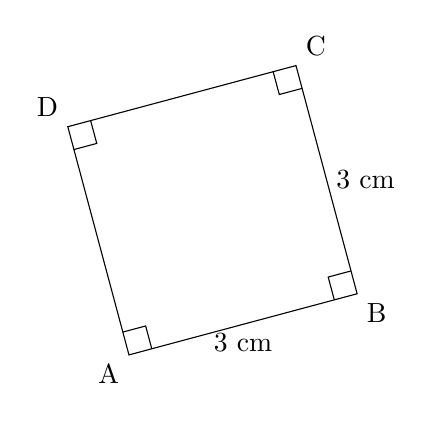
\begin{tikzpicture}
    \begin{scope}[rotate=15]
    \draw (0,0) coordinate (A) --
          ++(3,0) coordinate (B) --
          ++(0,3) coordinate (C) --
          ++(-3,0) coordinate (D) -- cycle;
    \foreach \p/\q/\r in {B/A/D,A/D/C,D/C/B,C/B/A} {
        \pic [draw, -, angle radius=0.3cm, angle eccentricity=1.6] {right angle=\p--\q--\r};
    }
    \path (C) -- node[right] {3 cm} (B);
    \path (A) -- node[below] {3 cm} (B);
    \foreach \p/\l in {A/below left,B/below right,C/above right,D/above left} {
        \node[\l] at (\p) {\p};
    }
    \end{scope}
\end{tikzpicture}
\end{minipage}%
\begin{minipage}{.4\textwidth}
\begin{align*}
\text{Area} &= \text{l}^2 \\
\text{Area} &= 3 \text{cm} \times 3 \text{cm}  \\
\text{Area} &= 9 \text{cm}^2
\end{align*}
\end{minipage}

\end{document}
